\section{Introduction}
\label{sec:introduction}

AI-assisted developers now generate code several times faster than they
can read it. A single engineer working with a coding assistant produces
pull requests that would previously have represented days of work, and
the bottleneck shifts from writing to reviewing. Reviewers have finite
attention and cannot inspect every line with equal care, yet the
failure modes of modern code generation concentrate in small, hard-to-%
spot places. Recent empirical work on deprecated APIs quantifies the
scale of the problem: LLM-based code completion emits deprecated API
calls at rates of roughly $25$--$38\%$ on standard prompts and
substantially more on legacy codebases, because the training corpus
straddles library-version transitions and the model has no posterior
knowledge of deprecation at inference time~\cite{wang2025deprecated}.

A reviewer facing AI-generated code has two problems, not one. The
first is \emph{which functions} to scrutinize; the second is \emph{where
within each function} to look. Existing uncertainty signals can answer
the first question: static analyzers catch known-bad patterns;
sequence-level confidence scores such as the mean token probability
\papg~\cite{spiess2025calibration} produce one number per function;
multi-sample methods~\cite{kuhn2023semantic,uqlm2024,sharma2025multisample}
re-roll the same prompt and measure output disagreement. None of them
answer the second. On a function the size of a non-trivial SDK call
--- roughly a hundred tokens --- the difference between ``flagged''
and ``flagged here, on this token, between these two alternatives''
is the difference between directing a reviewer and asking them to
re-read everything. Vasconcelos et
al.~\cite{vasconcelos2024genprob} provide direct human-subjects
evidence that this distinction matters in practice: in a controlled
user study, highlighting tokens by their probability of being edited
produced faster task completion and more targeted edits, while
highlighting tokens by raw generation probability produced no benefit.

\paragraph{A concrete instance.}
A model asked to charge a credit card might emit
\texttt{stripe.Charge.create(...)} --- deprecated since $2019$ --- or
\texttt{stripe.PaymentIntent.create(...)}, the current API. Both
arrive in the developer's editor with the same syntactic fluency, the
same confident indentation, and no visible marker distinguishing a
well-chosen call from one the model guessed at. At the method-%
selector token, the two choices split the probability mass near
50/50 ($P=0.52$ vs.\ $0.47$); the output exposes none of this. Failures
of AI code generation cluster at exactly these points: version-split
APIs, renamed SDK methods, signature changes between library releases.
The model is uncertain; the output is not.

\paragraph{Intra- versus inter-generational uncertainty.}
The gap between the internal split and a confident-looking output
is not an accident of any particular model; it is structural.
Multi-sample uncertainty quantification methods for LLMs are
\emph{inter-generational}: they sample the same prompt multiple
times and measure disagreement across completions~\cite{kuhn2023semantic,%
uqlm2024,sharma2025multisample}. This works when the model's
uncertainty surfaces as instability across re-rolls --- factual
questions, open-ended reasoning. Code is not such a task. A model
with a near-tie prior on the deprecated branch samples that branch
nearly every time; once the early tokens commit, the rest of the
function is forced by context. The uncertainty exists, but it
lives \emph{inside a single generation}, in the token distribution at
each decoding step, not \emph{across} generations. We call this the
\emph{intra- versus inter-generational} distinction.

\paragraph{\eps, and two levels at which it operates.}
We introduce \eps (epsilon), a per-token normalized Shannon entropy
over the top-$k$ log-probabilities returned during generation. After
AST-based filtering to keep only semantically meaningful tokens
(attribute accesses, keyword arguments, import targets --- not
whitespace, comments, or cosmetic identifiers), we aggregate via
max-pooling to obtain a single score per function. The function-level
score is a recall-maximizing filter: at threshold $\eps \ge 0.30$ it
flags $97\%$ of HIGH prompts with zero observed misses on
our evaluated benchmark set. A reviewer asked ``which functions need scrutiny''
gets a clear answer; at that scale, so does \papg. But the
function-level view discards most of what \eps knows. Of the
$\sim 98$ tokens in a typical flagged function, only $10.5\%$ exceed
the flag threshold. The same score that flags the function also tells
the reviewer that the relevant uncertainty lives in the method
selector on line $4$, not in the parameter block on lines $7$--$12$.
\eps is a two-level signal: a function-level filter that agrees with
\papg on ``which,'' and a token-level localizer that no sequence-level
aggregate can produce.

Figure~\ref{fig:token-focus-teaser} stages the full problem on Stripe
Scenario A (\S\ref{subsec:token-focus}): what the reviewer sees is a
single fluent line of code; what the model nearly emitted instead is
a near-tie with a different, currently-supported API; and where \eps
directs the review is to the few tokens within the $98$-token
function where that hesitation lives. The same score that flags the
function names the tokens that drove the flag.

\begin{figure}[H]
\centering
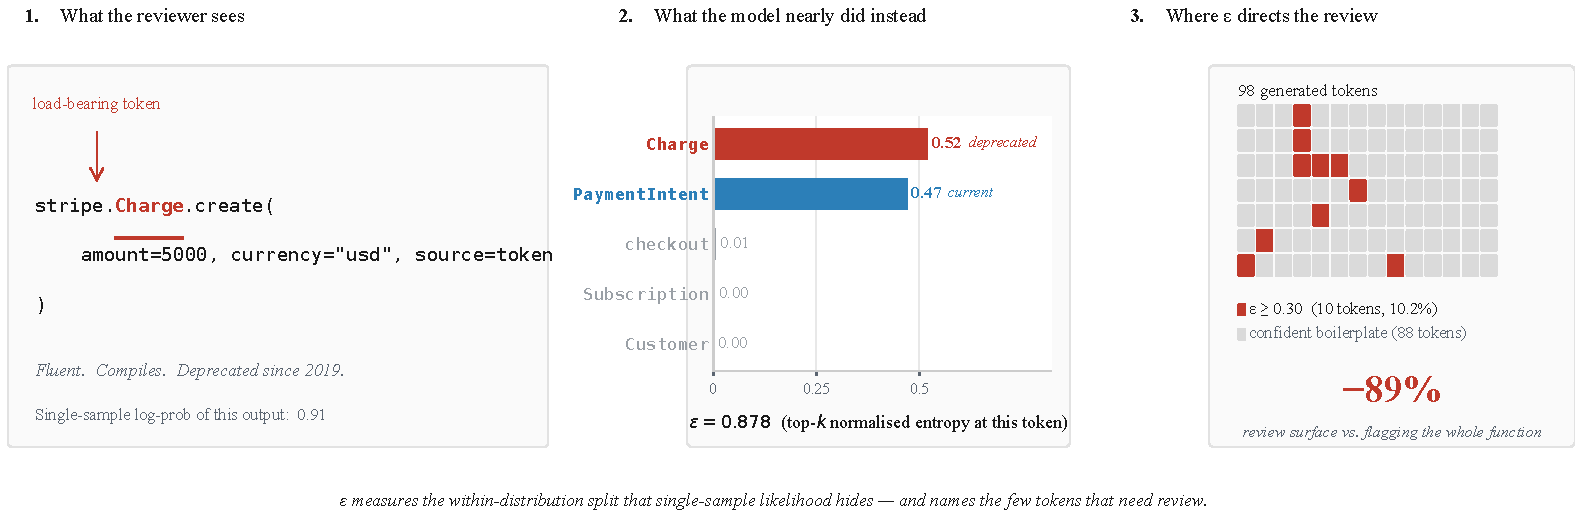
\includegraphics[width=\textwidth]{figures/fig_motivation.pdf}
\caption{The problem, the hidden distribution, and \eps's response,
on Stripe Scenario A (GPT-4o). \textbf{Left:} the reviewer sees a
fluent, compiling call to \texttt{stripe.Charge.create(\ldots)} ---
deprecated since $2019$ --- with a single-sample log-probability of
$0.91$. \textbf{Centre:} at the method-selector token, the top-$k$
distribution is a near-tie between \texttt{Charge} ($P=0.52$,
deprecated) and \texttt{PaymentIntent} ($P=0.47$, current); the
top-$k$-normalized entropy at this token is $\eps = 0.878$.
\textbf{Right:} of the $98$ semantic tokens in the function, $10$
($10.2\%$) exceed the flag threshold; the remaining $88$ are
confident boilerplate. \eps narrows the within-function review
surface by $89\%$ and points the reviewer at the specific tokens
that drove the flag. The paper-level claim in one image:
single-sample likelihood hides the within-distribution split that
\eps reads, and \eps names the few tokens that need review.}
\label{fig:token-focus-teaser}
\end{figure}

\paragraph{A three-way comparison.}
Because the function-level claim is not distinguishing, the
comparison in this paper is between \emph{signals}, not just detection
rates. We benchmark \eps against two alternatives at the same
$1\times$ API cost and one at $5\times$ on the same production-%
realistic prompts across four models. At $1\times$, the sequence-level
mean token probability \papg~\cite{spiess2025calibration} is
competitive with \eps on raw function-level detection
(\S\ref{sec:comparison}); what it cannot do is identify the specific
token at which the model was uncertain. \eps produces both the
function-level score and the token-level attribution. At
$5\times$ cost, multi-sample methods at $N=5$, $T=0.7$ detect
$10$--$35\%$ of HIGH prompts: the $52/47$ hesitation does not
surface as output variation, so inter-generational signals are
structurally blind to it. UQLM~\cite{uqlm2024}, the closest packaged
off-the-shelf tool, detects $5\%$ on the same benchmark.

\paragraph{The two-stage system.}
A $27\%$-precision filter is not meant to be used in isolation. Stage
$2$ is a parallel LLM review loop: every flagged entry is dispatched,
in parallel, to a reviewer model that returns \textsc{cleared} or
\textsc{confirmed}. The reviewer is not asked to re-read the whole
function. It is asked to examine the specific high-\eps tokens --- on
Stripe Scenario A, the handful of tokens whose \eps exceeds the flag
threshold. At current API prices this costs fractions of a cent per
entry and completes in seconds. The token-level attribution is not
decoration on the filter; it is the mechanism that makes the reviewer
fast and precise. On 201 entries across three models, a context-%
primed reviewer clears $68.7\%$ of flagged entries with zero late
false positives.

\paragraph{Contributions.}
\begin{enumerate}[noitemsep]
    \item The intra/inter-generational distinction, formalized and
    empirically verified: \eps reaches $85\%$ detection on GPT-4o and
    DeepSeek V3 against $10$--$35\%$ for direct multi-sample
    measurement and $5\%$ for UQLM on the same benchmark.
    \item Token-level localization as \eps's distinguishing claim:
    the function-level flag agrees with \papg; the token-level
    attribution is what no sequence-level signal can produce.
    \item A two-stage filter-plus-review architecture: $94\%$
    end-to-end precision on $201$ entries across three models, with
    the reviewer directed to high-\eps tokens.
    \item The first direct three-way empirical comparison --- \eps
    vs.\ \papg vs.\ multi-sample --- on production-realistic
    version-split prompts, isolating where each signal fires and
    where it does not.
\end{enumerate}

We use the labels \textsc{high} and \textsc{low} throughout:
\textsc{high} prompts are API/version-split tasks across Stripe,
OpenAI, SQLAlchemy, FastAPI, and Pydantic where an incorrect choice
causes functional failure; \textsc{low} prompts are pure-logic tasks
(sort, palindrome, Fibonacci, two-sum) where any correct algorithm
is functionally equivalent. A detailed calibration table appears in
\S\ref{subsec:calibration}.

Implementation and benchmark are at
\url{https://github.com/michaeljaquith/epsilon-code}.
